% easychair.tex,v 3.0 2011/10/24
%
% Select appropriate paper format in your document class as
% instructed by your conference organizers. Only withtimes
% and notimes can be used in proceedings created by EasyChair
%
% The available formats are 'letterpaper' and 'a4paper' with
% the former being the default if omitted as in the example
% below.
%
%\documentclass{easychair}
\documentclass[]{easychair}
%\documentclass[verbose]{easychair}
%\documentclass[notimes]{easychair}
%\documentclass[withtimes]{easychair}
%\documentclass[a4paper]{easychair}
%\documentclass[letterpaper]{easychair}
%\documentclass[notimes,custompaper,lmargin=1cm,rmargin=2cm,tmargin=.5cm,bmargin=1.5cm]{easychair}
%\documentclass[notimes,custompaper,lmargin=1cm,rmargin=2cm,tmargin=.5cm,bmargin=1.5cm]{easychair}

% This provides the \BibTeX macro
\usepackage{doc}
\usepackage{makeidx}

% In order to save space or manage large tables or figures in a
% landcape-like text, you can use the rotating and pdflscape
% packages. Uncomment the desired from the below.
%
% \usepackage{rotating}
% \usepackage{pdflscape}

% If you plan on including some algorithm specification, we recommend
% the below package. Read more details on the custom options of the
% package documentation.
%
% \usepackage{algorithm2e}

% Some of our commands for this guide.
%
\usepackage{xspace}
\usepackage{amssymb}
\usepackage{color}
\newcommand{\comment}[4]{\par\noindent\hspace*{-0.5cm}{\parbox{\columnwidth}{\textbf{\color{#1}//#2[#3]:#4}}}\par}

\newcommand{\easychair}{\textsf{easychair}}
\newcommand{\miktex}{MiK{\TeX}}
\newcommand{\texniccenter}{{\TeX}nicCenter}
\newcommand{\makefile}{\texttt{Makefile}}
\newcommand{\latexeditor}{LEd}
\newcommand{\ex}[1]{\emph{ex.}\xspace\emph{#1}}
\newcommand{\ie}[0]{\emph{c-à-d.}\xspace}
\newcommand{\mi}[1]{\comment{blue}{}{#1}{MI}}
\newcommand{\ch}[1]{\comment{green}{}{#1}{CH}}
\newcommand{\si}[1]{\comment{red}{}{#1}{SI}}
\newcommand{\FM}[0]{\textsc{fm}\xspace}
\newcommand{\Y}[0]{\textsc{YourCast}\xspace}
\newcommand{\LP}[0]{{ligne de produits}\xspace}
\newcommand{\LPS}[0]{{lignes de produits}\xspace}
\newcommand{\IR}[0]{interFMRelation}%\xspace}
\newcommand{\source}[0]{\textsc{source}\xspace}
\newcommand{\policy}[0]{\textsc{policy}\xspace}

%\makeindex

%% Document
%%
\begin{document}

%% Front Matter
%%
% Regular title as in the article class.
%
\title{Composition de workflows pour le filtrage sémantique d'informations}

% \titlerunning{} has to be set to either the main title or its shorter
% version for the running heads. Use {\sf} for highlighting your system
% name, application, or a tool.
%
\titlerunning{workflows et filtrage sémantique}

% For only the editors. Authors, please keep this commented out
% \volumeinfo
% 	{G. Sutcliffe, A. Voronkov}         % editors
% 	{2}                                 % number of editors
%	{{\easychair} 3.0 Beta 5, March 2011}      % event
%	{2}                                 % volume
%	{1}                                 % issue
%	{1}                                 % starting page number
%\indexededitor{Sutcliffe, Geoff}
%\indexededitor{Voronkov, Andrei}

%\headfootstyle
%	{}
%	{\sf}
%	{\footnotesize\sf}
%	{\small}

\volumeinfoECPS
	{CIEL Proceedings}
	{ECPS vol. 7999}

% Authors are joined by \and and their affiliations are on the
% subsequent lines separated by \\ just like the article class
% allows.
%
\author{
    Christophe Desclaux\\
    \affiliation{Université Nice Sophia-Antipolis}\\
    \affiliation{\url{christophe@zouig.org}}\\
\and
    Simon Urli\\
    \affiliation{I3S, CNRS}\\
    \affiliation{Université Nice Sophia-Antipolis}\\
    \affiliation{\url{urli@i3s.unice.fr}}\\
\and
    Mireille Blay-Fornarino\\
    \affiliation{I3S, CNRS}\\
    \affiliation{Université Nice Sophia-Antipolis}\\
    \affiliation{\url{blay@polytech.unice.fr}}\\
\and
    Catherine Faron Zucker\\
    \affiliation{I3S, CNRS}\\
    \affiliation{Université Nice Sophia-Antipolis}\\
    \affiliation{\url{faron@polytech.unice.fr}}\\
}

% \authorrunning{} has to be set for the shorter version of the authors' names;
% otherwise a warning will be rendered in the running heads.
%
\authorrunning{C. Desclaux, S. Urli, M. Blay-Fornarino and C. Faron Zucker}
\indexedauthor{Christophe, Desclaux}
\indexedauthor{Simon, Urli}
\indexedauthor{Mireille, Blay-Fornarino}
\indexedauthor{Catherine, Faron Zucker}

%%%%%%%%%%%%%%%%%%%%%%%%%%%%%%%%%%%%%%%%%%%%%%%%%%%
\maketitle
%%%%%%%%%%%%%%%%%%%%%%%%%%%%%%%%%%%%%%%%%%%%%%%%%%%
%------------------------------------------------------------------------------
% Abstract
%
\begin{abstract}
Le web se révèle aujourd'hui un merveilleux support de diffusion d'informations. Tandis que les sources se multiplient (flux rss, services web, ..), la quantité d'informations croît et il est difficile de les filtrer en fonction de nos centres d'intérêts. Actuellement de nombreux outils qui exploitent les ontologies ou les thésaurus sont mis au point. Ils permettent d'annoter les informations, d'en déduire des critères et d'ensuite obtenir uniquement les informations pertinentes. La composition de ces outils constitue des workflows qui devraient encore s'enrichir grâce à l'apparition de nouvelles ontologies ciblées sur différents domaines et outils de lecture.  Cependant la construction de telles chaînes logicielles n'est pas à la portée de tous. \\
Dans cet article nous montrons comment de tels workflows ont été construits et présentons nos perspectives en matière de construction automatique de ces workflows en fonction des besoins utilisateur. Ce travail s'appuie sur le projet ANR EMergence Yourcast qui vise à automatiser la diffusion des informations sur de grands écrans, et pour lequel la pertinence des informations diffusées est donc particulièrement pertinent. 
\end{abstract}

\begin{abstract}
Internet is becoming today a wonderful medium for disseminating information. While the sources are multiplying (RSS, WebServices, ...), the amount of information is growing and it's difficult to filter them according to our interests. Currently many tools that exploits ontologies or thesauri are developed. They help us to annotate informations and to derive criteria and then get only the relevant information. The composition of these tools constitute workflows that should be enriched by the emergence of new ontologies focused on different domains and text analysis tools. However the composition of this tools-chain is not for everyone.\\
In this paper we show how these workflows have built and present our outlook for the automated build of workflows based on user needs. This work is supported by the ANR Emergence Yourcast project designed to automate the dissemination of information on large screens, and for which the relevance of the information published is particularly relevant.
\end{abstract}
%------------------------------------------------------------------------------

\section{Présentation et importance du filtrage des informations dans le web de données}
\label{sect:introduction}

Le web se révèle aujourd'hui un merveilleux support de diffusion des informations. Tandis que les sources se multiplient (flux rss, services web, ..), la quantité des informations croît et il est difficile de les filtrer en fonction de nos centres d'intérêts  \cite{Bouzeghoub2005}. Des outils qui exploitent les ontologies ou les thésaurus dans le web sémantique \cite{Lee2001} ont été mis au point qui permettent d'annoter les informations, d'en déduire des critères et d'ensuite obtenir uniquement les informations pertinentes. 
\mi{enrichir ce qui précède avec des références en essayant si possible de faire ressentir les éléments de l'architecture.}

Il devient aujourd'hui possible de construire à la fois des workflows mettant en jeux ces différents outils pour annoter les flux d'informations  puis les sélectionner les informations. 
Cependant la construction de ces workflows reste technique malgré les nouveaux supports logiciels tels que les mashup \cite{Floyd2007} \cite{Milanovic2004}. En effet elle se base sur de nombreux critères qui doivent être pris en compte pour assembler les services et le fait que ces services soient hétéroclites ne permet pas une génération aisée des applications. De plus de nouvelles ontologies, sources, systèmes d'annotations apparaissent régulièrement tandis que le web se démocratise \cite{Anderruthy2007} \cite{Bross2010} \mi{et surtout bien le dire}. 
Dans ce contexte, la production automatique de ces workflows à partir d'un ensemble de caractéristiques proposées à l'utilisateur apparaît comme d'une grande utilité. 

Dans cet article, en section \ref{sect:exemple}  nous présentons un cas d'étude qui a été mené dans le cadre projet ANR EMergence Yourcast qui vise à automatiser la diffusion des informations sur de grands écrans. Nous montrons au travers de ce cas d'étude les différents choix qui se posent à l'utilisateur \mi{MOntrer cela} et décrivons dans la section \ref{sect:miseEnOuvre} les workflows  mis en place pour répondre à ce cas particulier. Fort de cette expérience, nous proposons en \ref{sect:perspectives} de produire de tels workflows en utilisant un développement dirigé par les modèles et les feature models pour produire automatiquement de tels workflows à partir de données utilisateur de haut niveau. 


%------------------------------------------------------------------------------

\section{Système de diffusion des informations sur grands écrans et filtrage}
%ch : etat de l'art de notre appli, présentation du problème (outils à utiliser solutions, exploitation et de qu'on aimerait faire. chalenges!
\label{sect:exemple}
\mi{Clairement je cherche le titre...}
Dans le cadre du projet \Y, nous visons à diffuser sur de grands écrans des informations en provenance de différentes sources en particulier celles issues du web. Or de tels systèmes exigent une adhérence forte aux attentes des utilisateurs et l'adéquation des informations avec les centres d'intérêts des personnes est essentielle à l'acceptation de tels systèmes. 

\paragraph*{Des sources hétérogènes}
Or il existe aujourd'hui de nombreuses sources d'information disponibles grâce à l'utilisation de flux RSS \cite{Lassila}. Le choix des sources peut être simplement lié au travail ou à l'emplacement géographique de l'écran d'information.
Dans notre cas, nous avons choisi d'agréger le plus de sources d'informations possible pour couvrir tous les champs d'application des écrans d'accueil. 
Nous faisons donc appel dans notre application à une vingtaine de flux rss sur de vastes sujets. Ceux-ci sont essentiellement des flux aillant déjà subit une étape de filtrage qui a permis de les classer selon leurs thématique générale (technologies, international, médical...).

\paragraph*{Sélections des informations}
Beaucoup de sources d'informations sont agrégeables. Des critères de sélection sont alors pré-établis par les fournisseurs de contenus.  Par exemple sur le site de news de google \url{http://news.google.fr} vous pouvez accéder à des nouvelles liées à l'économie ou bien les news locales. Cependant  vous ne pouvez pas récupérer les news économiques liées à la ville de Marseille ou plus largement à la région PACA. Dans notre exploitation des flux RSS nous devons donc pouvoir fournir un filtrage multi-critères permettant un tri fin des informations. 

\paragraph*{Des critères utilisateurs}
Pour capturer ces critères il existe différents systèmes actuellement tel que le service \url{http://www.google.fr/reader/} ou bien \url{http://rsslounge.aditu.de} cependant ceux-ci ne proposent pas de regroupement des flux et de filtrage multi-critère de ceux-ci.
En effet, nous avions besoin d'un système intuitif qui permet de capturer simplement les exigences utilisateur. Nous avons choisis sur ce point un système d'aide au choix que nous avons construit et qui après captation en langage naturel des besoins les retranscrit sous forme d'entités nommées qui sont typées par notre système en fonction des éléments que nous avons déjà pu instancier dans la base de connaissances.

\paragraph*{Des processus d'annotation diversifié}
Le système est basé sur une annotation des informations la plus vaste possible. En effet le système doit pouvoir annoter des informations provenant de domaines totalement différents.
Nous avons choisis d'utiliser des annotions basées sur la récupération d'entités nommées présentes sur un grand nombre de bases de données RDF (Resource Description Framework \cite{Winer2005}).
Nous utilisons alors des systèmes d'extraction d'information et d'annotation sémantique qui permettent d'ajouter des liaisons vers les entités nommés spécifiques.


%------------------------------------------------------------------------------

\section{Mise en œuvre}
\label{sect:miseEnOuvre}
Dans le cadre de l'étude présentée précédemment nous avons donc mis au point deux workflows, dont nous présentons à présent l'architecture brièvement. Comme présenté sur le diagramme suivant nous avons ainsi le workflow d'enrichissement des informations (coloré en bleu ainsi que le workflow de filtrage des informations.

\begin{figure}[htb!]
	\begin{centering}
	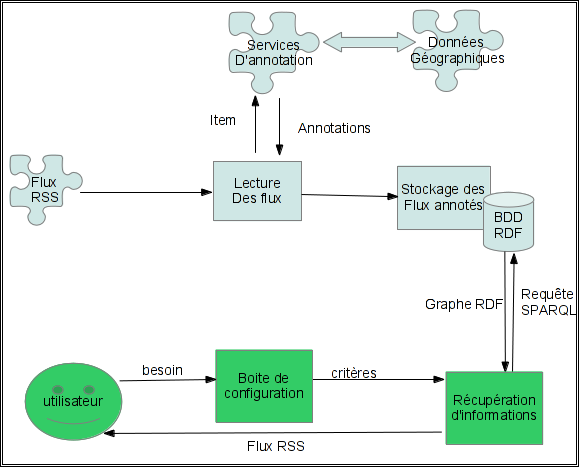
\includegraphics[width=0.7\textwidth]{diagramme-Archi.png}
	\caption{Workflow de traitements....}
	\label{fig:mmFM}
	\end{centering}
\end{figure}

\subsection{Workflow d'enrichissement des informations}
Nous allons nous attarder particulièrement sur ce workflow car il fait appel à de nombreux services d'annotation et nécessite une modularité dans l'organisation de ceux-ci.

\subsubsection{Lecture de flux RSS}
L'application se base sur la récupération de flux RSS qui sont choisis par l'utilisateur et dont nous connaissons le thème et la langue, chaque flux rss va contenir un lot de news les plus récentes publiées chez le fournisseur du flux. Le flux peut être mis à jour et nous devons l'interroger périodiquement pour récupérer les dernières informations publiées.

\subsubsection{Annotation }
Sur chaque news nous devons utiliser les services d'annotation pour récupérer les entités nommées intéressantes le concernant. Pour cela nous faisons appel à divers services d'annotation qui nous renvoient les informations. Nous avons aussi besoin de faire appel à des services de généralisation qui vont travailler en aval des services d'annotation pour ajouter des notions à une annotation.\\
De manière concrète nous utilisons les services d'annotation suivants:
\begin{itemize}

\item Services d'Annotation
\begin{itemize}
\item \textbf{OpenCalais} nous permet de récupérer les entités des textes correspondant à des lieux français ainsi que des noms de personnalités en langue anglaise. Nous lui indiquons en entrée le texte à annoter et récupérons une liste de mots correspondant à nos critères.
\item \textbf{WikiMeta} fonctionne de la même manière qu'OpenCalais mais permet de récupérer directement des entités nommées pointant vers la base de connaissance DBpedia, il peut donc être utilisé seul en tant que service d'annotation principal
\end{itemize}

\item Services de Généralisation
\begin{itemize}
\item \textbf{DBpedia} travaille sur les données provenant du service d'annotation WikiMeta et permet de les enrichir sémantiquement à l'aide de liens vers d'autres ressources liées à l'élément
\item \textbf{INSEE geo} \url{http://rdf.insee.fr/geo/} La base de données RDF de l'INSEE nous permet de récupérer les ensembles géographiques liées à une entité nommée géographique. Ce service d'annotation géographique s'utilise donc uniquement en aval d'un service d'annotation classique qui récupère des informations géographiques. Il renvoi en sortie des URI vers les entités géographiques liées à la news étudiée. Nous utilisons pour cette interrogation la requête SPARQL suivante qui permet d'avoir les informations désirées:

\begin{verbatim}
PREFIX geo: <http://rdf.insee.fr/geo/>
SELECT = DISTINCT = ?nom ?type WHERE{
	 ?entite geo:nom ?nom
	 ?entite rdf:type ?type
	 { 
		  ?ville geo:nom ?nomVille
		  ?entite geo:subdivision* ?ville
		  ?FILTER(regex(str(?nomVille), ‘Nice’, ‘i’))
	}
}
\end{verbatim}
\end{itemize}

\end{itemize}

\subsubsection{Mémorisation}
\mi{je ne sens pas cette partie.. à voir}
Nous stockons le contenu des flux RSS et les annotations dans une base de données RDF grâce à l'utilisation de l'application 4Store. 4store est un serveur de triplets RDF fournissant un accès aux données en lecture et écriture. Il nous permet de créer un EndPoint en ligne rapide et puissant. De plus, cela permet une réutilisation de notre travail d'annotations dans d'autres projets aillant besoin d'accéder à des flux annotés. Enfin cette technologie va permettre une excellente connection entre le workflow d'enrichissement et celui de filtrage car de nombreuses APIs existent pour attaquer la base de données dans différents langages.

\subsection{Workflow de filtrage des informations}
Le workflow de filtrage permet de créer des critères utilisateurs affin de récupérer les données intéressantes sur la base de données. Chaque critère est défini par le couple (TypeDeRelation, EntitéeNommée) et va permettre un choix précis des éléments à récupérer. Nous fournissons une application complète permettant de choisir les critères à appliquer sur la base \cite{Christophe}.
%on choisi de ne pas détailler ce workflow

%------------------------------------------------------------------------------

\section{Perspective : Vers la construction automatique de workflows }
\label{sect:perspectives}
Notre objectif à terme est de construire une ligne de produits qui capturerait les différents sources et systèmes d'annotation disponibles, les qualifierait et permettrait à un utilisateur final de construire ses propres workflows d'annotation en sélectionnant pour lui les sources et les systèmes d'annotations idoines conformément à ses choix.

\subsection{Objectifs et limites}

La construction automatique de workflows d'annotations permet de répondre à différentes problématiques. Du point de vue de l'utilisateur final, l'utilisation d'une construction de workflows pourrait lui permettre, à partir d'un flux sélectionné, d'affiner la sélection des services d'annotations qu'il souhaite utiliser afin d'obtenir l'information la plus complète pour son utilisation.

En outre, à l'heure actuelle le workflow d'annotation interroge tous les services d'annotations disponibles, sans distinction de catégories, ce qui génère de nombreux appels de service dont la plupart sont inutiles. L'utilisation d'une construction automatique à partir des choix de l'utilisateur permettrait de restreindre les appels aux seuls services pertinents et donc d'accélérer les temps de traitements en réduisant la charge des services. 

Nous limitons dans cette expérimentation les choix de l'utilisateur aux seules notions de \textit{Thèmes} et de \textit{Langues} en raison de leur pertinence et de leur impact sur la sélection des sources et des systèmes d'annotations. En effet, soient les systèmes d'annotations sont directement spécialisés pour certains types d'informations, comme le service MetaMap \cite{MetaMap} spécialisé dans l'annotation de données médicales, soit ils fournissent une API permettant de restreindre les annotations à certaines catégories d'informations, certains \textit{Thèmes}. Par ailleurs, la langue est un critère déterminant pour annoter correctement les informations, les systèmes d'annotations n'en supportent ainsi qu'un nombre limité. 

Enfin, les travaux présentés dans cette section sont en cours de recherche et n'ont pas encore fait l'objet d'une implémentation concrète.

\subsection{Lignes de produits de services}
Les choix que va faire l'utilisateur vont avoir un impact sur trois concepts inhérents aux workflow d'annotations : les \textit{Flux} d'information, les \textit{Services d'Annotation} et les \textit{Services de Généralisation}. Chacun de ces concepts peut être pris comme une ligne de produit indépendante, représentée par un feature model (FM) afin d'exprimer la variabilité des différents concepts.
\si{Réf FM / SPL - Expliquer choix de la SPL ?}

La figure ... montre ainsi le FM de \textit{Service d'Annotation} : les produits finaux correspondent aux feuilles de la feature \textit{Product}, les thèmes aux feuilles de la feature \textit{Thème} et les langues à celles de la feature \textit{Langue}. La sélection d'une feature de langue ou de thème influe directement sur le choix d'un produit final par le jeu des contraintes internes au FM. 

\si{à voir si on garde en dessous...}
Chacun des FM des différents concepts est une construction réalisée à partir d'une approche bottom-up. Nous partons des produits existants, en les exprimant sous forme de FM individuels, puis nous effectuons la fusion de ces FM afin d'obtenir une SPL modélisant les différents produits disponibles ainsi que leur variabilité \cite{Acher2011}.

\subsection{Modèle de mise en relation des LPL}
Notre but est de fournir un outil permettant à un utilisateur final de sélectionner des services cohérents en fonction de ses choix. Cela implique que chaque choix que l'utilisateur fera dans un des FM, doit avoir un impact sur les autres concepts du domaine. 

Comme le montre la figure ...., nous exprimons donc des relations entre les différents concepts du domaine, relations qui s'expriment - comme nous l'avons introduit - essentiellement sur le \textit{Thème} et la \textit{Langue}. La notion de relation a ici une double signification : elle va tout d'abord exprimer qu'un concept va être lié à un ou plusieurs autres concepts, en fonction de la cardinalité de la relation.

Par exemple, un \textit{Flux} va être annoté par un ou plusieurs \textit{Service d'annotation}, et chaque service d'annotation peut ensuite faire appel à un ou plusieurs \textit{Service de généralisation} afin d'améliorer la qualité des annotations. De façon réflexive, un \textit{service de généralisation} peut également en appeler un unique autre afin d'être encore plus fin.

Cependant, la relation permet également d'exprimer une restriction sur les choix de l'utilisateur : elle force que la sélection d'un produit dans un FM soit compatible avec la sélection d'un autre produit. En effet, la sélection d'un flux d'un certain thème et d'une certaine langue doit contraindre l'utilisateur à ne pouvoir sélectionner que les services d'annotations capables d'annoter des informations dans cette langue et sur ce thème. 

Cela est possible par la définition et l'application d'une opération de restriction sur les FMs liés entre eux en cascade. Par exemple, dans le cadre de la relation entre les \textit{Flux} et les \textit{Service d'Annotation}, un service d'annotation ne peut annoter un flux que s'ils s'expriment dans la même langue et parlent des mêmes thèmes. Ainsi, l'opération de restriction, pour la langue, consistera ici à déselectionner automatiquement dans un FM les langues ne correspondant pas au choix de l'utilisateur. 

Par exemple, si un produit du FM \textit{Flux} est spécifié être en Français, la sélection de ce produit sélectionnera automatiquement la feature \textit{Fr} par le jeu des contraintes internes. La restriction associée à la relation \textit{Flux-Service d'Annotation} va avoir pour effet de déselectionner toutes les features filles de \textit{Langue} et par le truchement des relations internes, de déselectionner les produits associés à ces langues. Il ne restera donc plus à l'utilisateur que la possibilité de sélectionner un service spécifique au français (\textit{Fr}).


Ainsi, la sélection d'un produit dans un FM va automatiquement induire l'indisponibilité de certains produits dans les FM liés. Or cette opération va elle même engendrer de nouvelles restrictions : en effet, la déselection d'un produit dans un FM peut également engendrer la déselection d'un autre produit dans un autre FM par le truchement des relations. 
\ch{parler certainement de la notion de cascade ici}
Cependant il est important de noter que chacune de ces opérations de restriction correspond à un contexte spécifique aux sélections de l'utilisateur dans les différents FM. En effet, l'utilisateur doit avoir la possibilité de sélectionner plusieurs produits dans chacun des FM : il va certainement souhaiter utiliser plusieurs services d'annotations différents pour un flux, ou au contraire souhaiter sélectionner plusieurs flux pour un même service d'annotation. Dans ces deux exemples différents, nous nous situons à chaque fois dans un contexte précis, le contexte de la sélection d'un flux spécifique, ou encore le contexte de la sélection d'un service d'annotation spécifique. Les opérations de restriction vont toujours s'exprimer dans un contexte spécifique tels que ceux-ci, mais l'utilisateur doit toujours avoir la possibilité de faire une nouvelle sélection, à partir d'un contexte vide. 

\subsection{Vers la génération des codes}
\ch{on supprime cette partie la non?}

\paragraph{}
Lien Asset / FM 

\paragraph{}
Construction de Workflow à partir du modèle

\paragraph{}
Lien workflow / code ?


%---------------------------------------------------------------
\section{Conclusion}
\label{sect:conclusion}



%------------------------------------------------------------------------------
% Refs:
%
\label{sect:bib}
\bibliographystyle{plain}
%\bibliographystyle{alpha}
%\bibliographystyle{unsrt}
%\bibliographystyle{abbrv}
\bibliography{christophe}

%------------------------------------------------------------------------------
\appendix

%------------------------------------------------------------------------------
% Index
%\printindex

%------------------------------------------------------------------------------
\end{document}

% EOF
